\documentclass{beamer}
\usepackage{graphicx}
\usepackage{xcolor}
\usepackage[normalem]{ulem}
\usepackage{mathtools}
\usetheme[titlepagelogo=firenze,% Logo for the first page
		  language=italian,
		  bullet=circle,
		  color=blue,
         ]{TorinoTh}
\usepackage[beamer,customcolors]{hf-tikz}
\definecolor{UniBlue}{RGB}{83,121,170}
\uselanguage{english}
\languagepath{english}
\setbeamercolor{block title}{use=structure,fg=white,bg=UniBlue}
\setbeamercolor{block body}{use=structure,fg=black,bg=white}

\author{}
\rel{{\normalsize Lorenzo Cioni}}
\title{\huge Illuminant maps analysis for image splicing detection}
\date{27 April 2017}

\begin{document}

\titlepageframe

%-- Intro --%

\begin{tframe}{Introduction}

\vspace{0.5cm}
Digital images are easy to manipulate thanks to the availability of the \textbf{powerful editing software} and \textbf{sophisticated digital cameras}.

\vspace{1cm}

\begin{minipage}{\textwidth}
\begin{columns}[T]
\begin{column}{0.46\textwidth}
\vspace{0.1cm}
The development of methods for verifying \textbf{image authenticity} is a real need in forensics.

\vspace{0.8cm}
\textbf{Purpose}: to detect image splicing  aimed at \emph{deceiving} the viewer.
\end{column}
\begin{column}{0.45\textwidth}
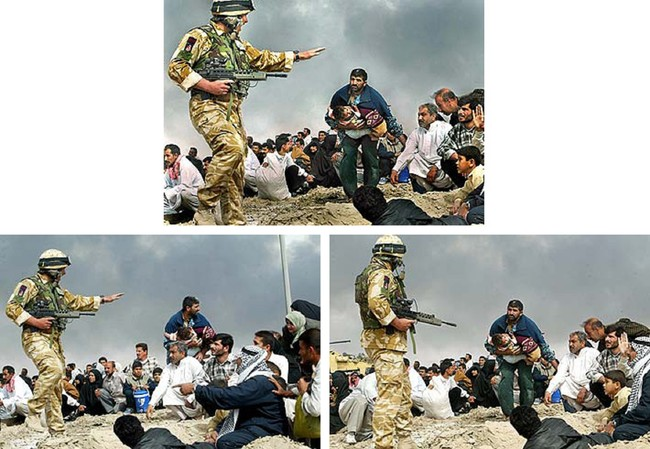
\includegraphics[width=1\textwidth]{images/iraq.jpg}
\end{column}
\end{columns}
\end{minipage}

\end{tframe}

%-- Image compositions --%

\begin{tframe}{Forgery detection approaches}

\vspace{0.2cm}
Image forensic detection techniques search for \textit{traces}, called \emph{footprints}, that can be grouped into:
\vspace{0.3cm}
\begin{enumerate}
\item \textbf{\textit{Signal} level}: signal specific properties left during the editing phase that can be revealed using signal processing-based tools.
\vspace{0.3cm}
\item \textbf{\textit{Scene} level}: exploiting inconsistencies in scene shadows, lights, reflections, perspective, and geometry of objects. \textit{Main advantage}: being fairly independent on low-level characteristics of images, they are extremely robust to compression, altering, and other image processing operations
\end{enumerate}
\vspace{0.3cm}
\end{tframe}

%-- Light based detection --%

\begin{tframe}{Lighting-based inconsistencies}
Methods based on \textbf{lighting inconsistencies} are particularly \emph{robust}: a perfect illumination adjustment in a image composition is very hard to achieve.
\begin{center}
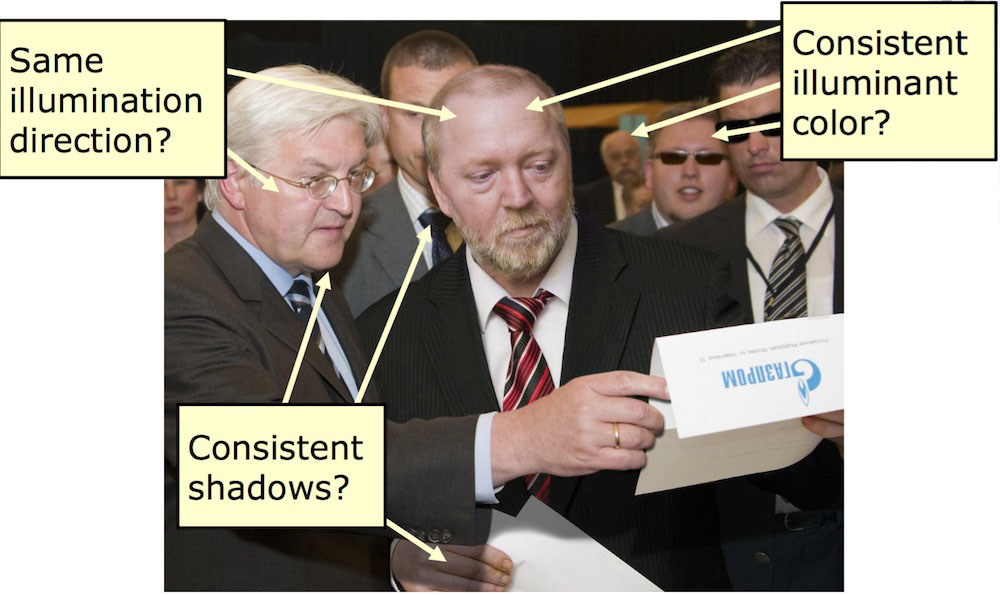
\includegraphics[width=0.4\textwidth]{images/lighting-based.jpg}
\end{center}
\begin{enumerate}
\item \textbf{Object light source inconsistencies}
\vspace{0.1cm}
\item \textbf{Illuminant colors inconsistencies}
\vspace{0.1cm}
\begin{enumerate}
\item \textit{Specular dichromatic reflectance models} {\tiny (Gholap and Bora, 2008 [5])}
\vspace{0.1cm}
\item \textbf{\uline{Illuminant Maps (IMs)}}
\end{enumerate}
\end{enumerate}
\vspace{0.3cm}
\end{tframe}


\begin{tframe}{Illuminant Maps estimation}
\vspace{0.2cm}
For the \emph{Illuminant Maps} estimation, two different \emph{state-of-art} techniques are used: 
\vspace{0.3cm}
\begin{small}
\begin{enumerate}
\item A \emph{statistical-based} approach using \textbf{Generalized Grayworld Estimate (GGE)} algorithm {\tiny (Van de Weijer \emph{et al.}, 2007 [3])}. Rely on hypotheses related to statistics of image pixels (e.g.  the \emph{gray world assumption}).
\vspace{0.2cm}
\item A \emph{physics-based} approach using \textbf{Inverse-Intensity Chromaticity (IIC)} method {\tiny (Riess and Angelopoulou, 2010 [4])}. Rely on theoretical formulations of how light interacts with objects (e.g. \emph{the dichromatic reflectance model})
\end{enumerate}
\end{small}

\begin{center}
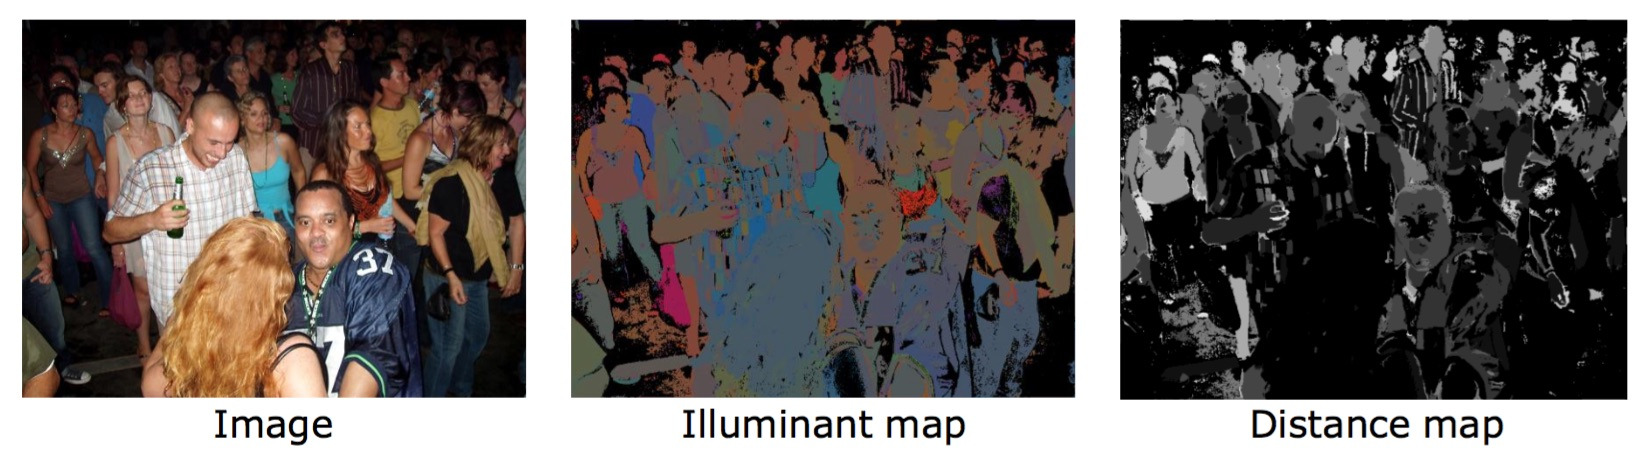
\includegraphics[width=0.55\textwidth]{images/riess.jpg}
\end{center}

\end{tframe}

\begin{tframe}{Proposed approach}
\uncover<1->{The current \emph{state of the art} approaches requires human interaction. }\uncover<2->{
$$\Downarrow$$
\vspace{-1cm}}
\uncover<3->{
\begin{center}
\textbf{Main goal}: \emph{remove the Human from the Loop}
\end{center}
Two different starting points:
\vspace{0.1cm}
\begin{itemize}
\item \textbf{Face forgery detection module}: specifically for detecting forgeries involving people. Based on the work presented by Carvalho \emph{et al. }2016 [1]. Improving and automating the detection process.

\item \textbf{Regional forgery detection module}: image content independent. Based on the work presented by Fan \emph{et al.} in 2015 [2]. A more general and experimental approach.
\end{itemize}}
\end{tframe}

\begin{tframe}{Face forgery detection module - 1}
\only<1>{
\begin{center}
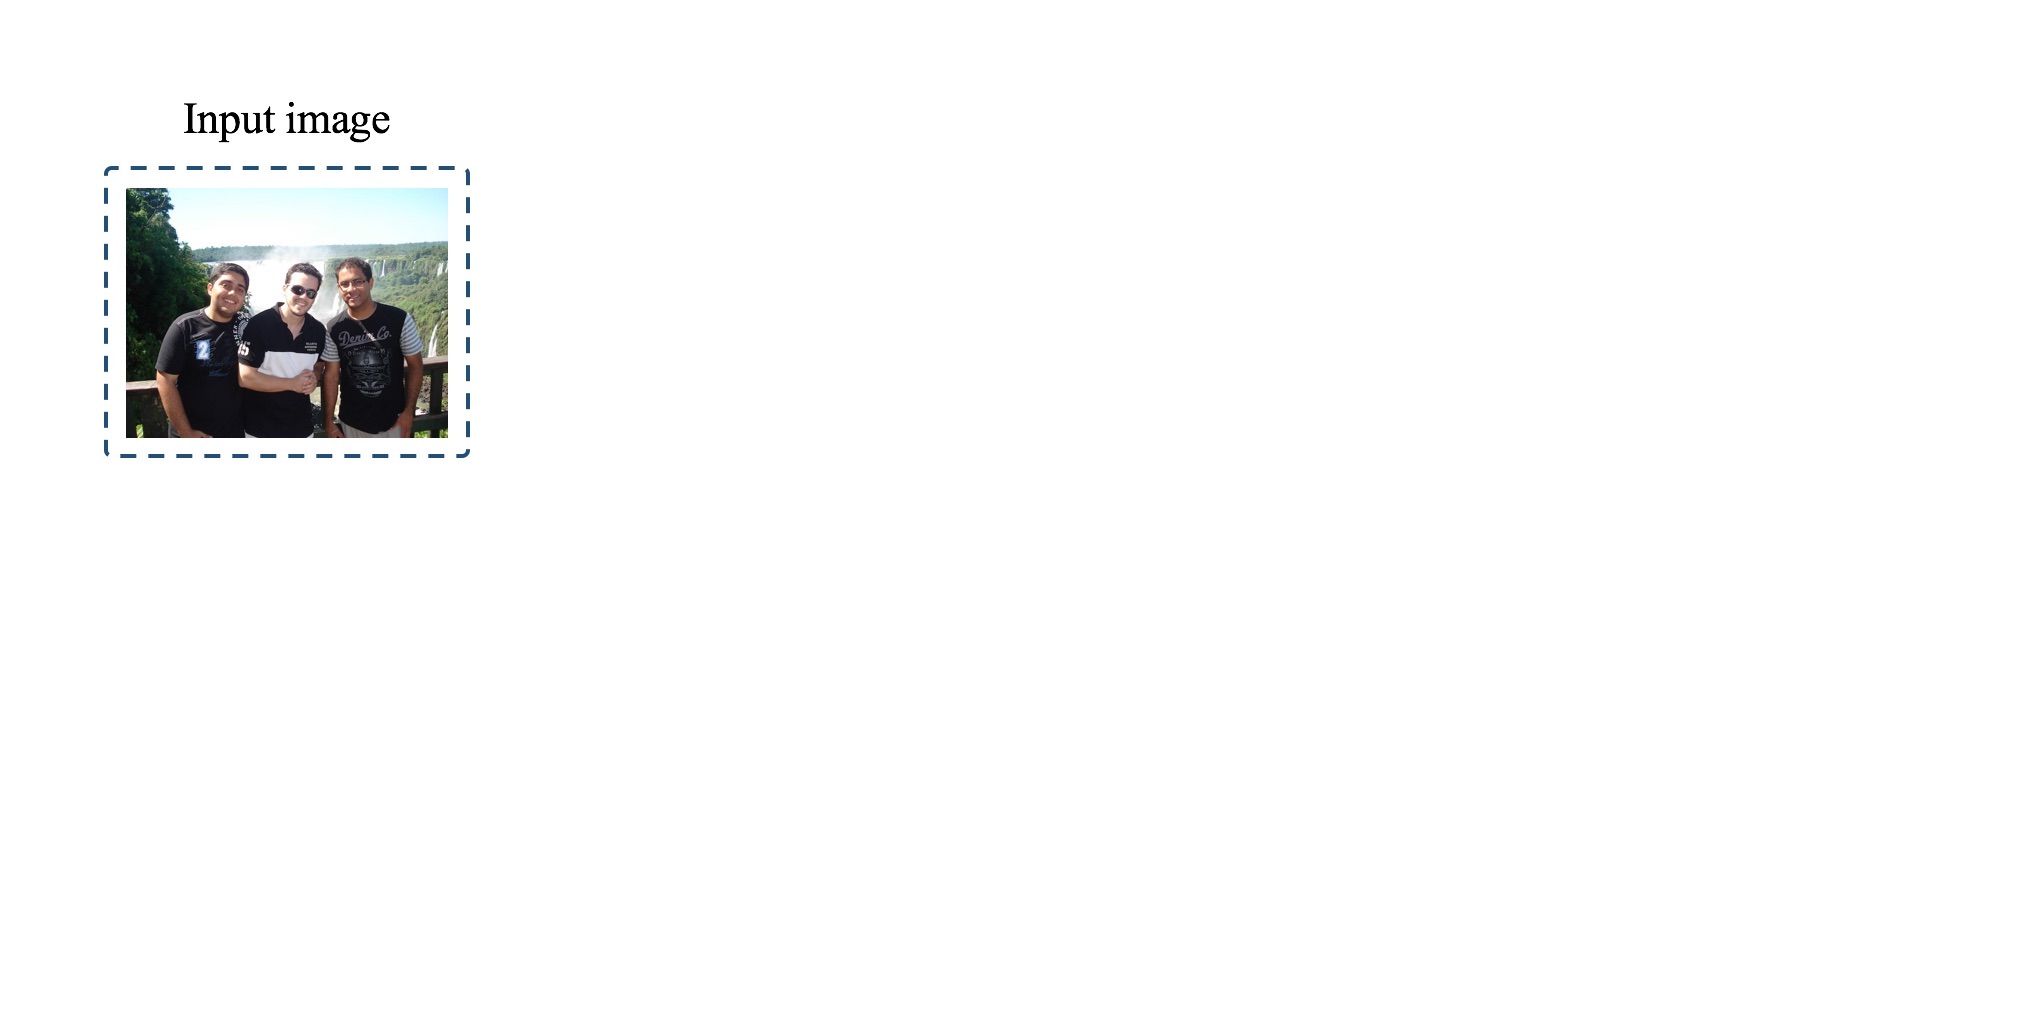
\includegraphics[width=1\textwidth]{images/pipeline_faces_1.jpg}
\end{center}
}
\only<2>{
\begin{center}
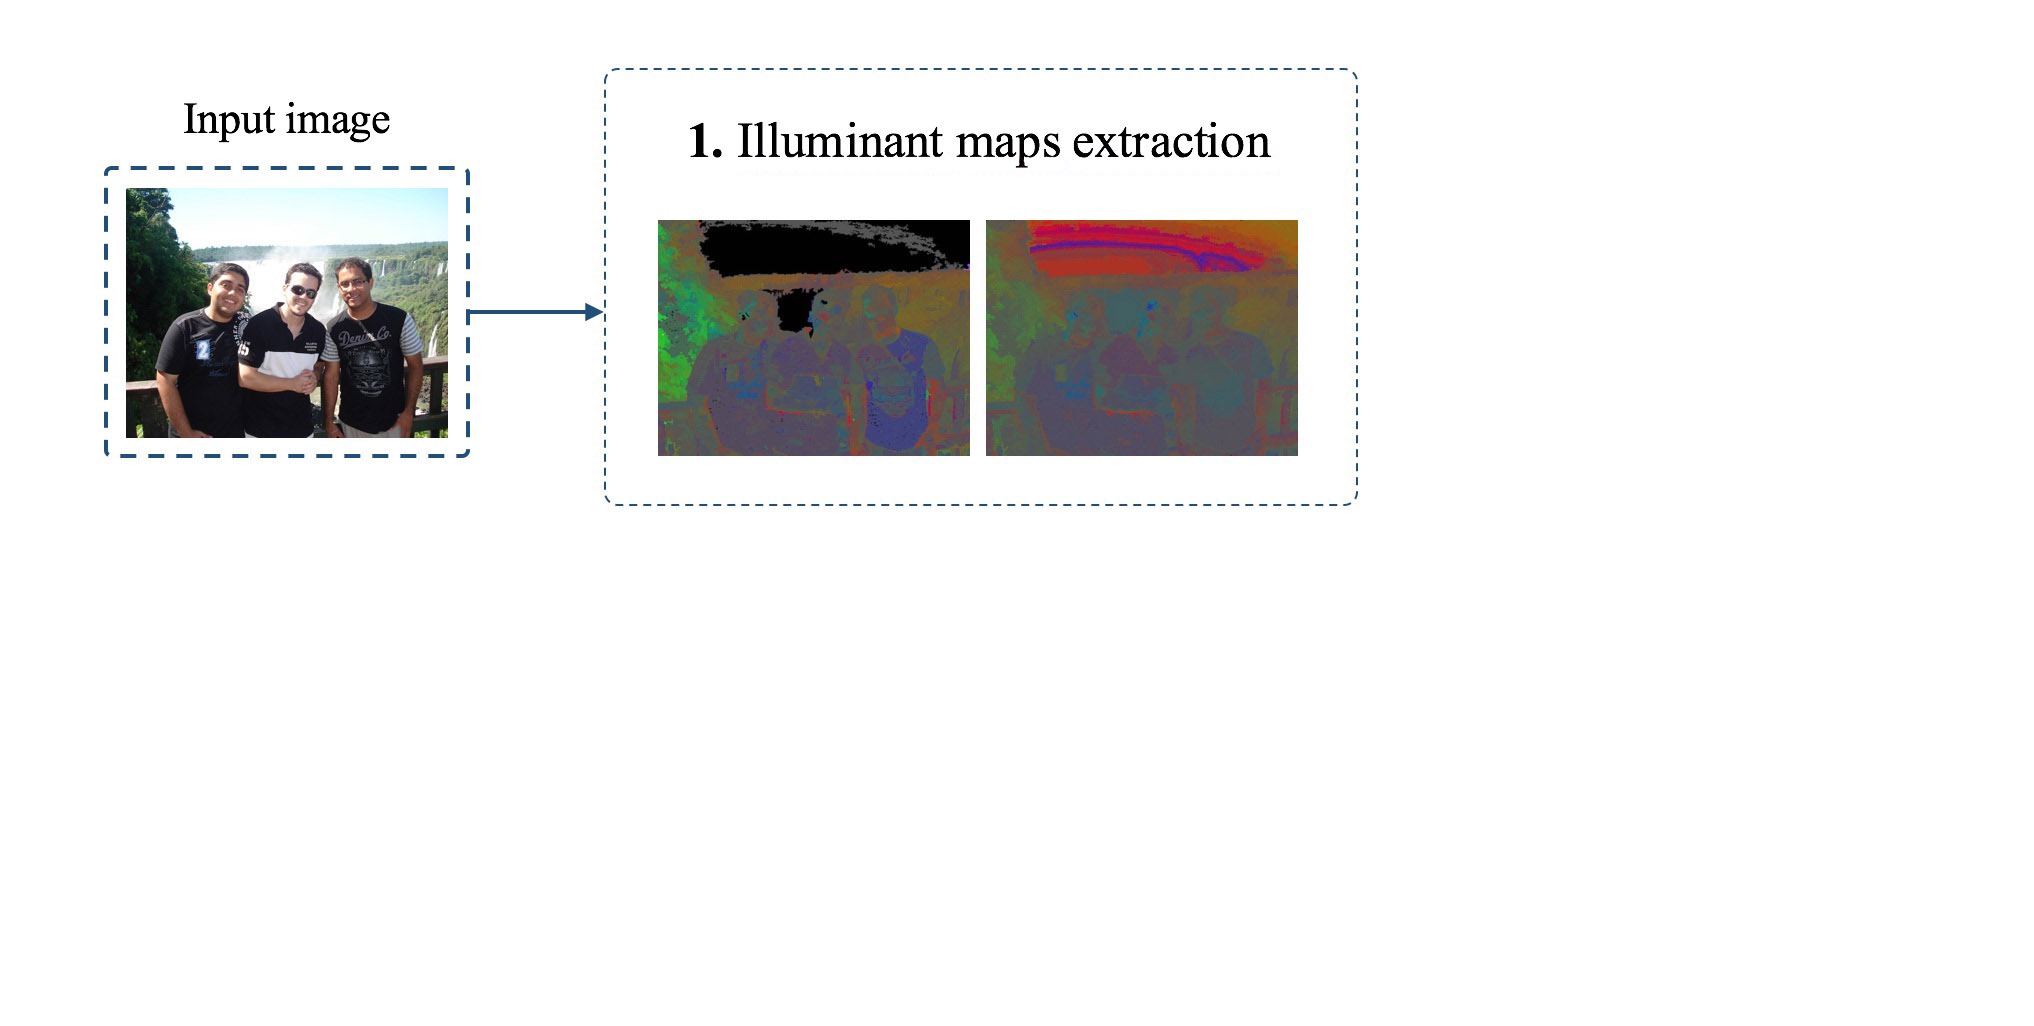
\includegraphics[width=1\textwidth]{images/pipeline_faces_2.jpg}
\end{center}
}
\only<3>{
\begin{center}
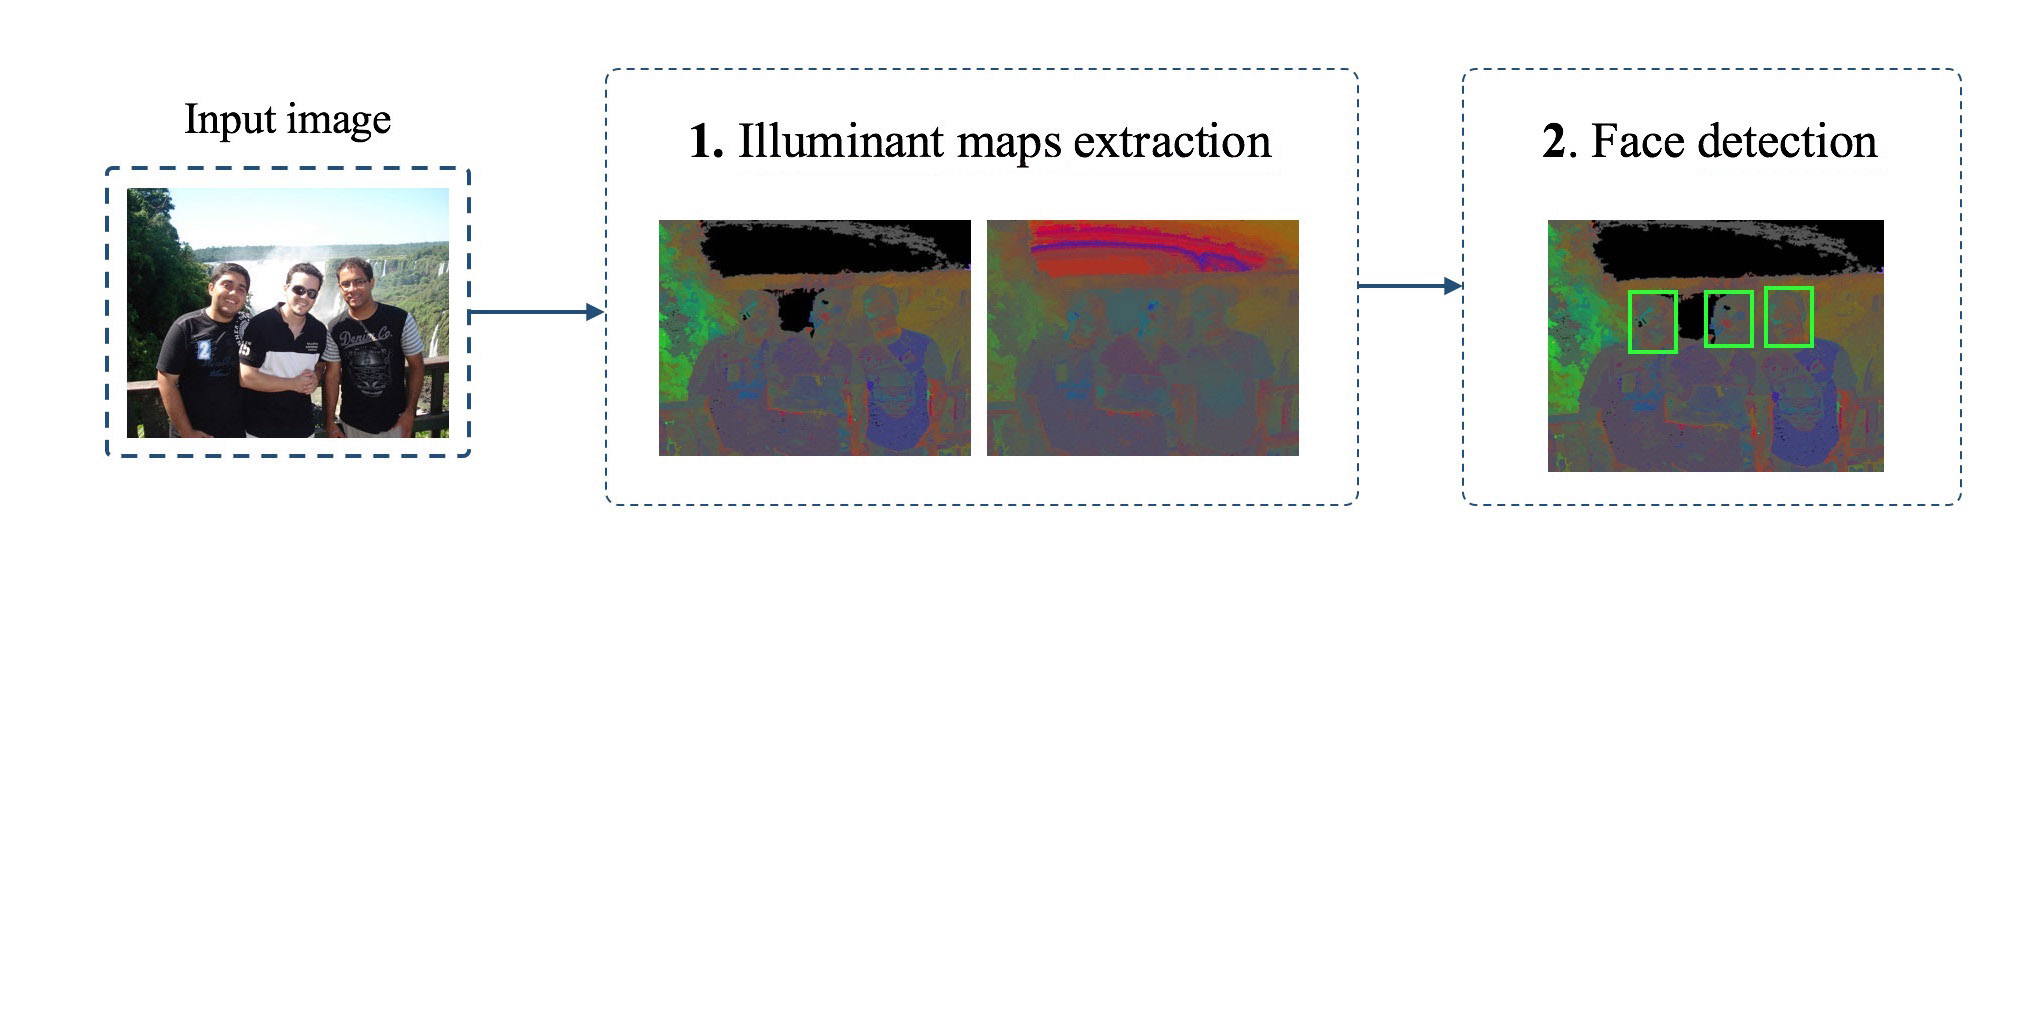
\includegraphics[width=1\textwidth]{images/pipeline_faces_3.jpg}
\end{center}
}
\only<4>{
\begin{center}
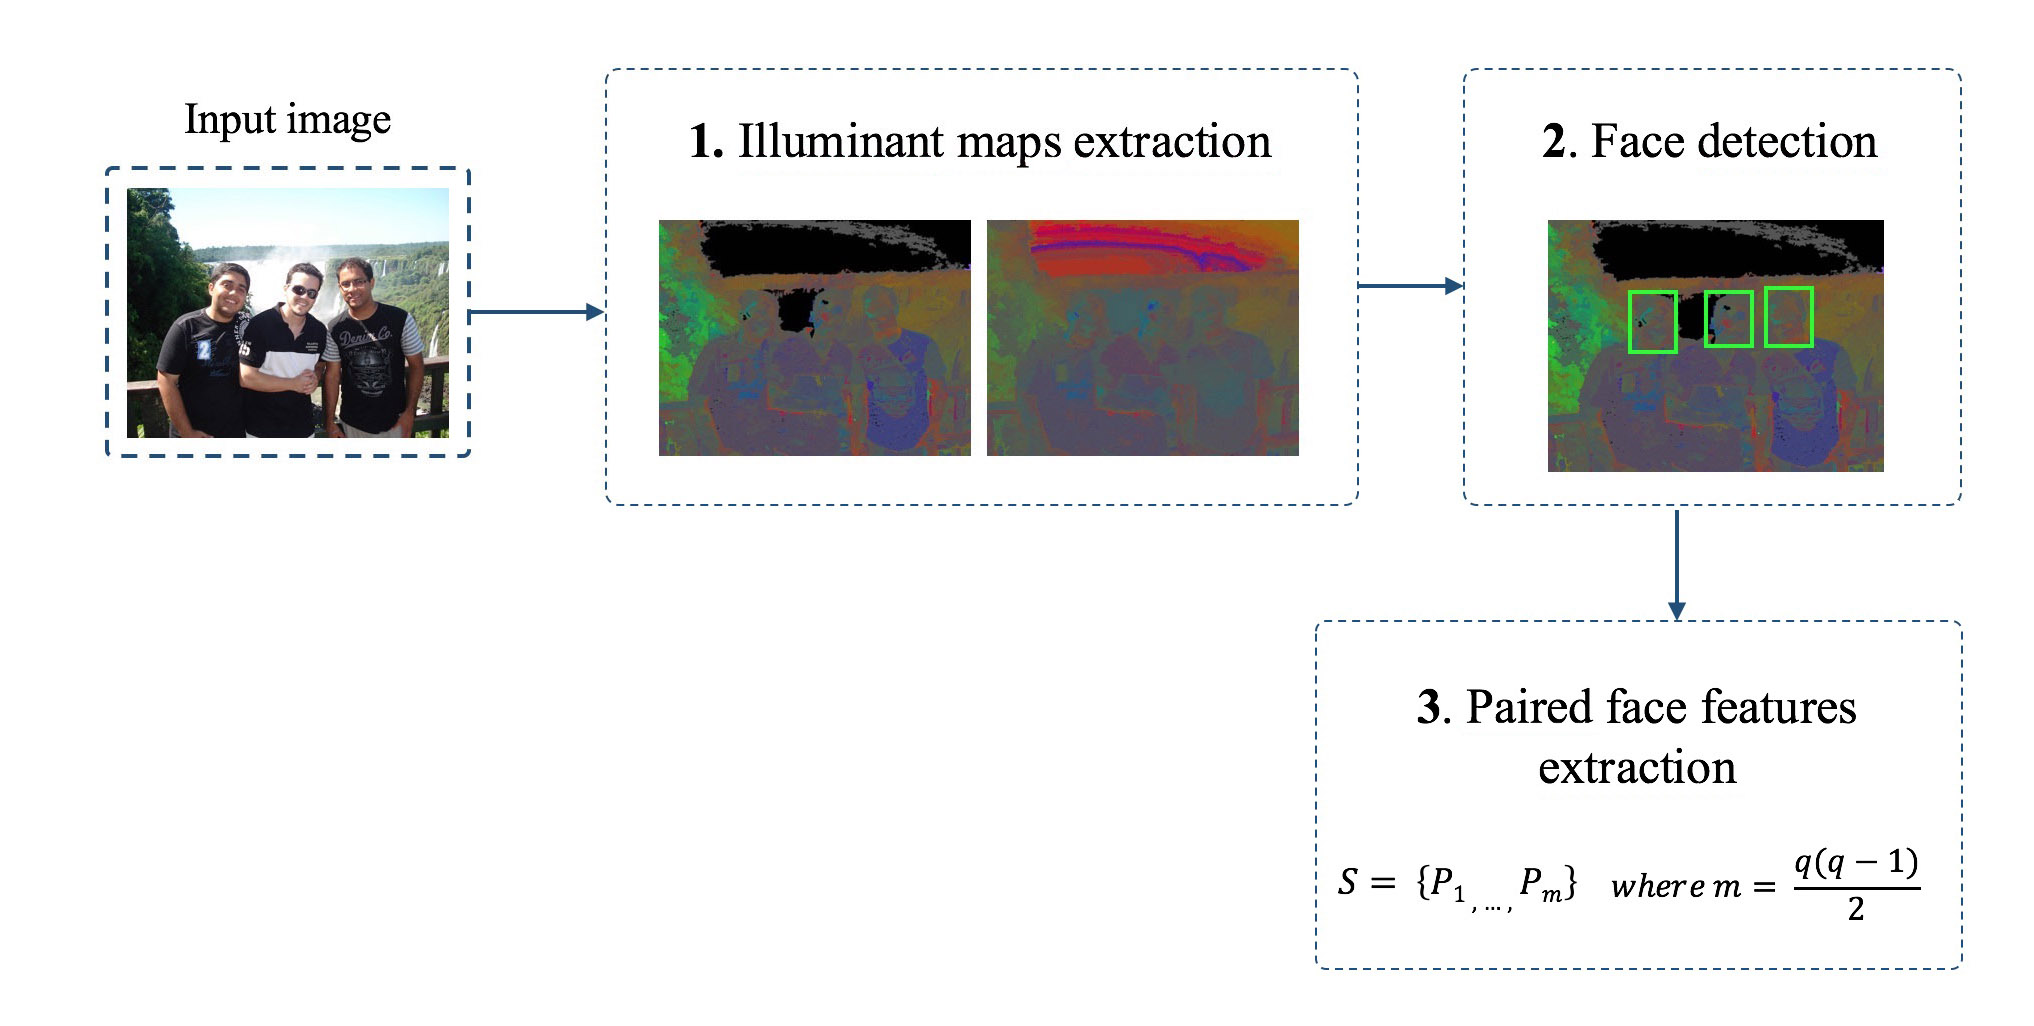
\includegraphics[width=1\textwidth]{images/pipeline_faces_4.jpg}
\end{center}
}
\only<5>{
\begin{center}
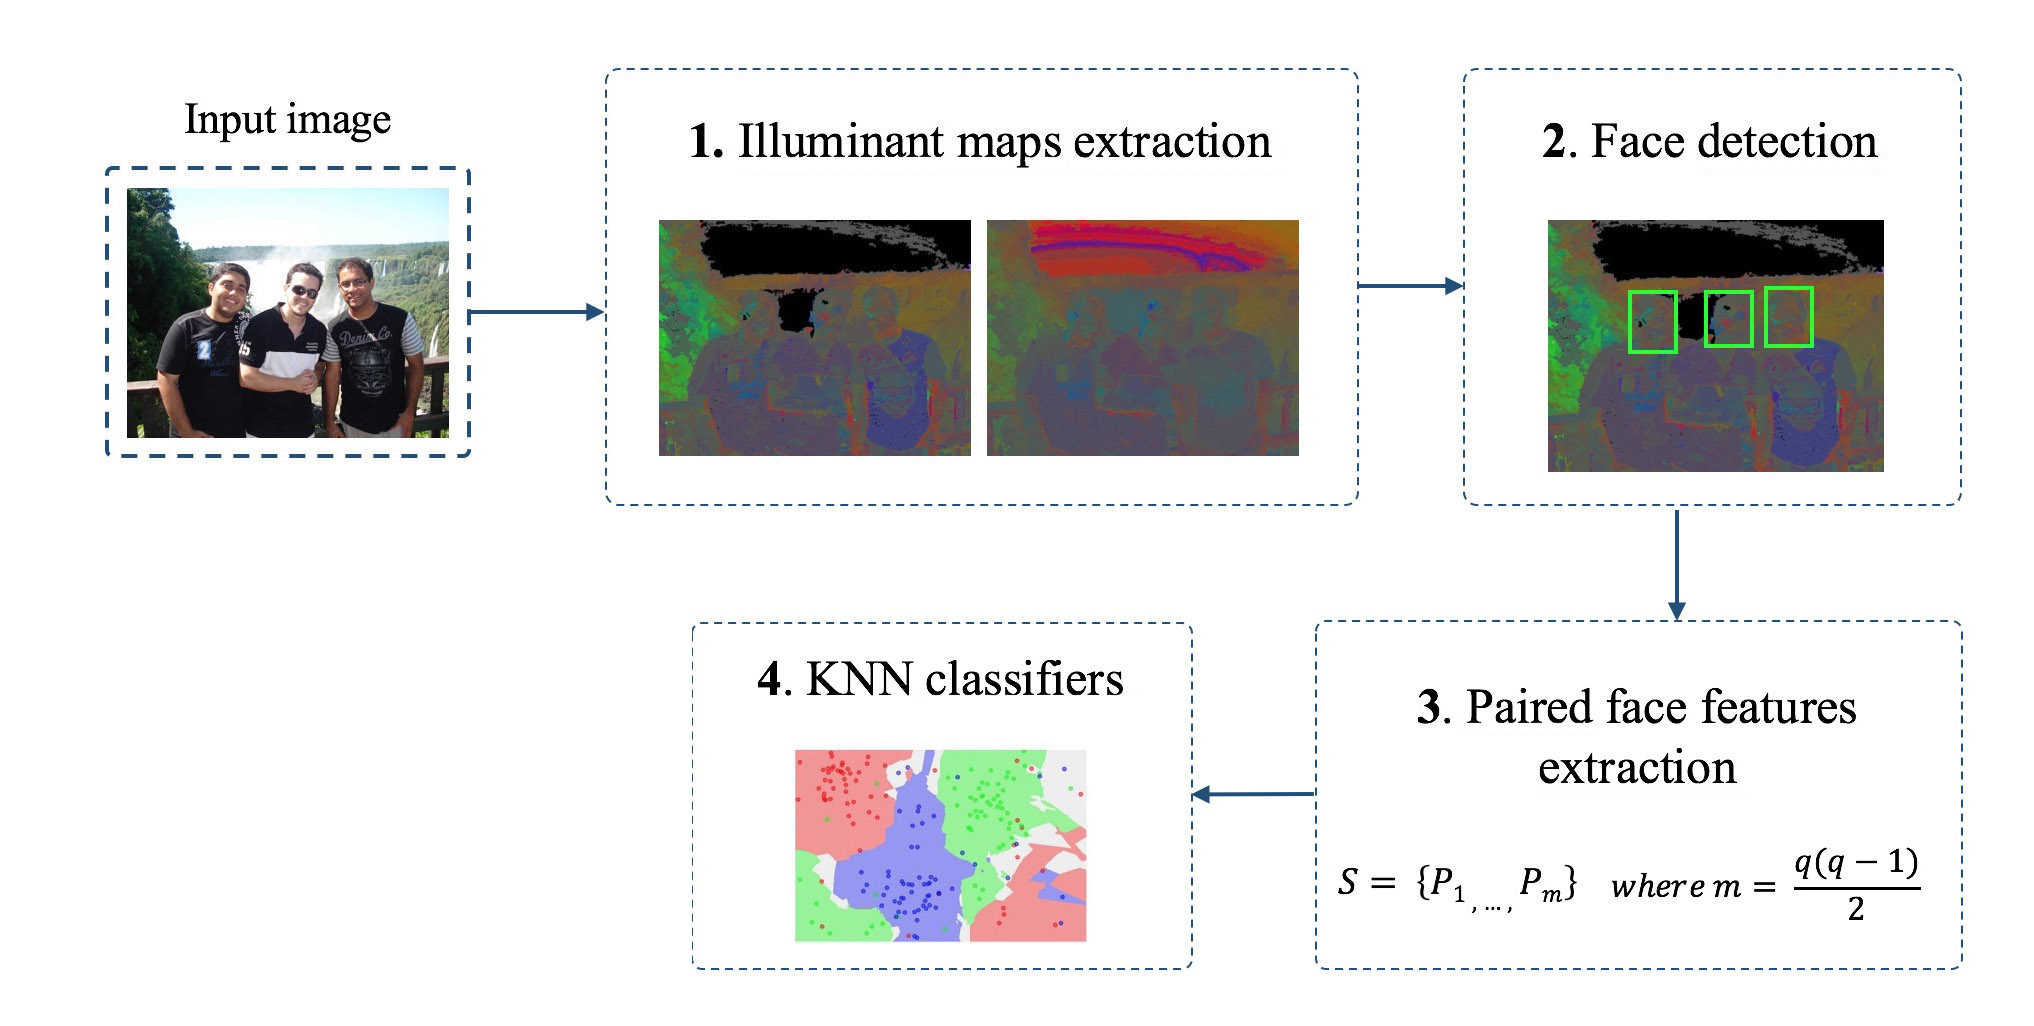
\includegraphics[width=1\textwidth]{images/pipeline_faces_5.jpg}
\end{center}
}
\only<6->{
\begin{center}
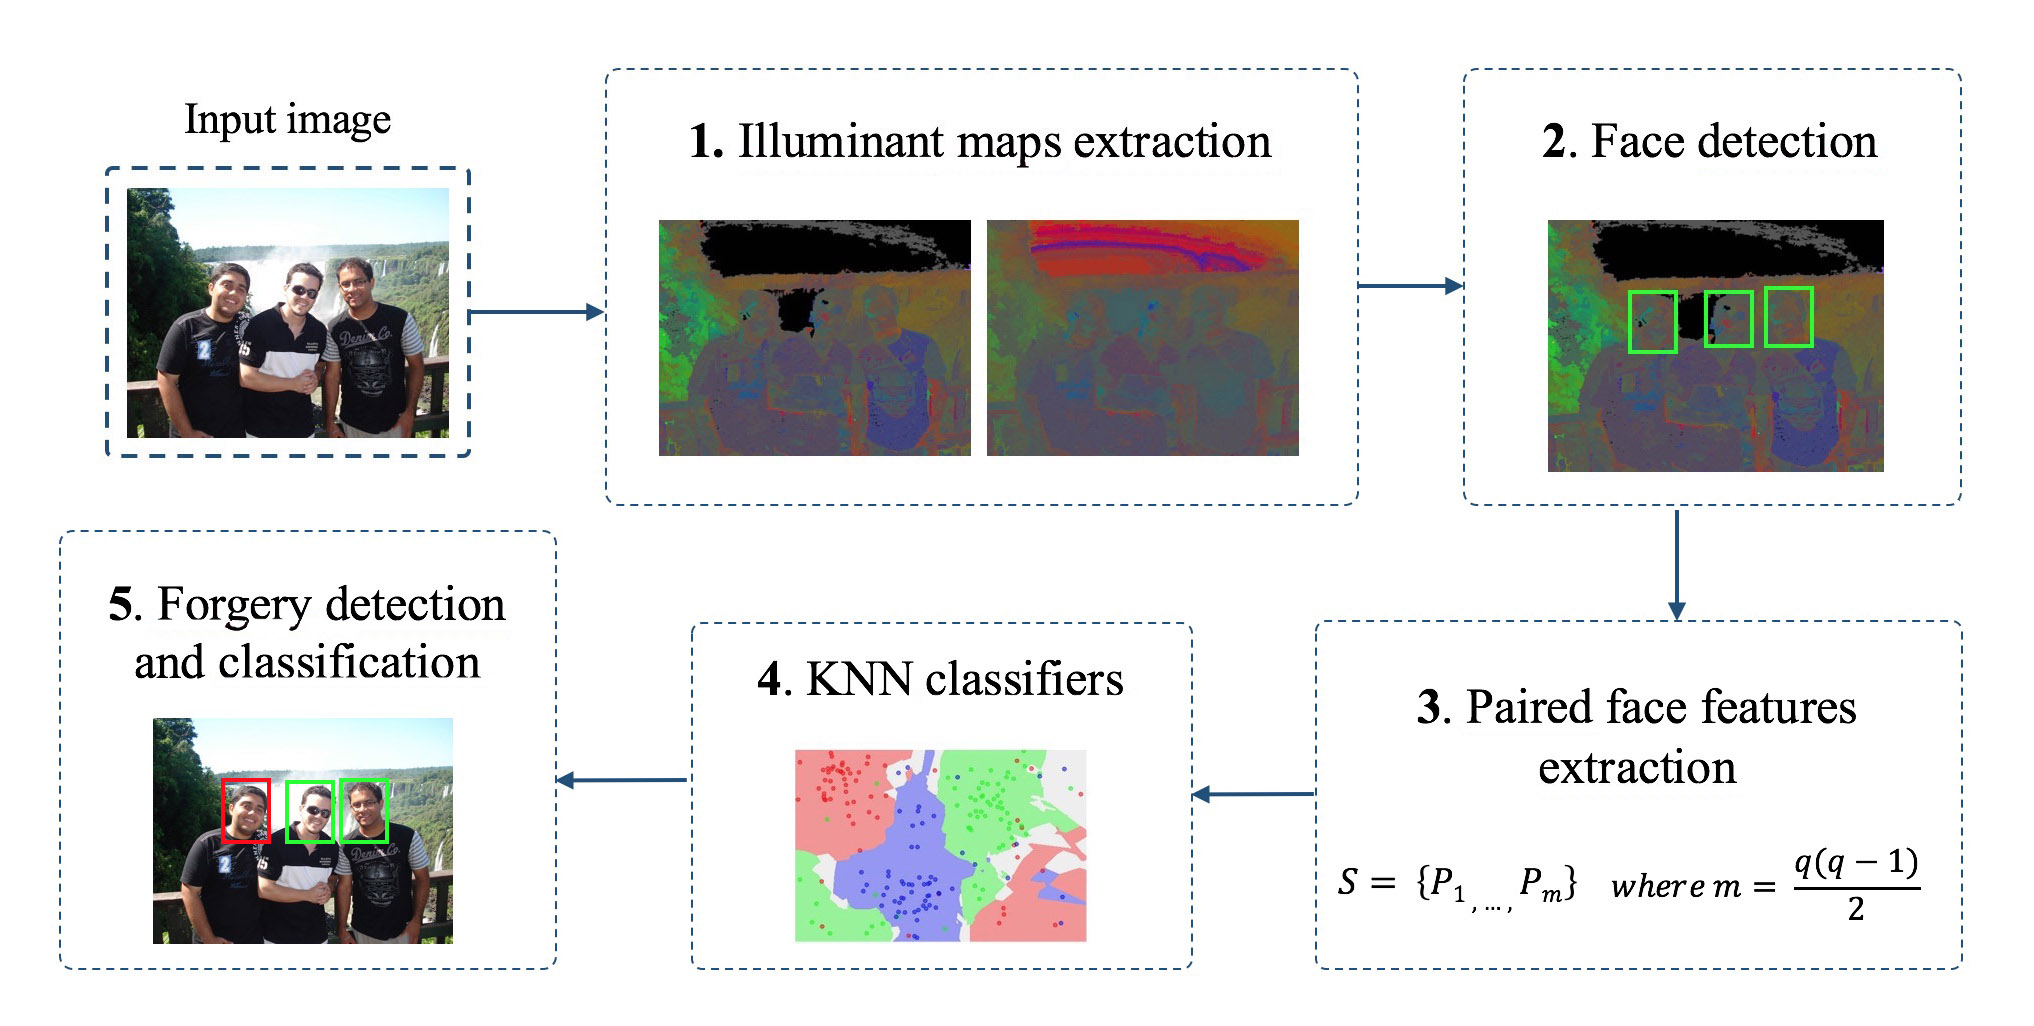
\includegraphics[width=1\textwidth]{images/pipeline_faces_6.jpg}
\end{center}
}
\only<7>{
Introducing a \emph{face detector} and \emph{soft classification scores}.
}
\end{tframe}


\begin{tframe}{Face forgery detection module - 2}
\vspace{0.1cm}
The output of the algorithm consist in a \textbf{forgery score} for each detected face.

\vspace{0.2cm}
\begin{minipage}{\textwidth}
\begin{columns}[T]
\begin{column}{0.2\textwidth}

\vspace{1cm}
\begin{center}
\begin{table}[h!]
\centering
\begin{tabular}{l c} 
\hline \hline 
\textbf{Face} & \textbf{Score}\\ [0.5ex]
\hline
A & 0.354\\
B & 0.354\\
C &	0.375\\
D &	0.396\\
\textbf{E} & \textbf{0.936}\\[1ex]
\hline
\end{tabular}
\end{table}
\end{center}
\end{column}
\begin{column}{0.7\textwidth}
\begin{center}
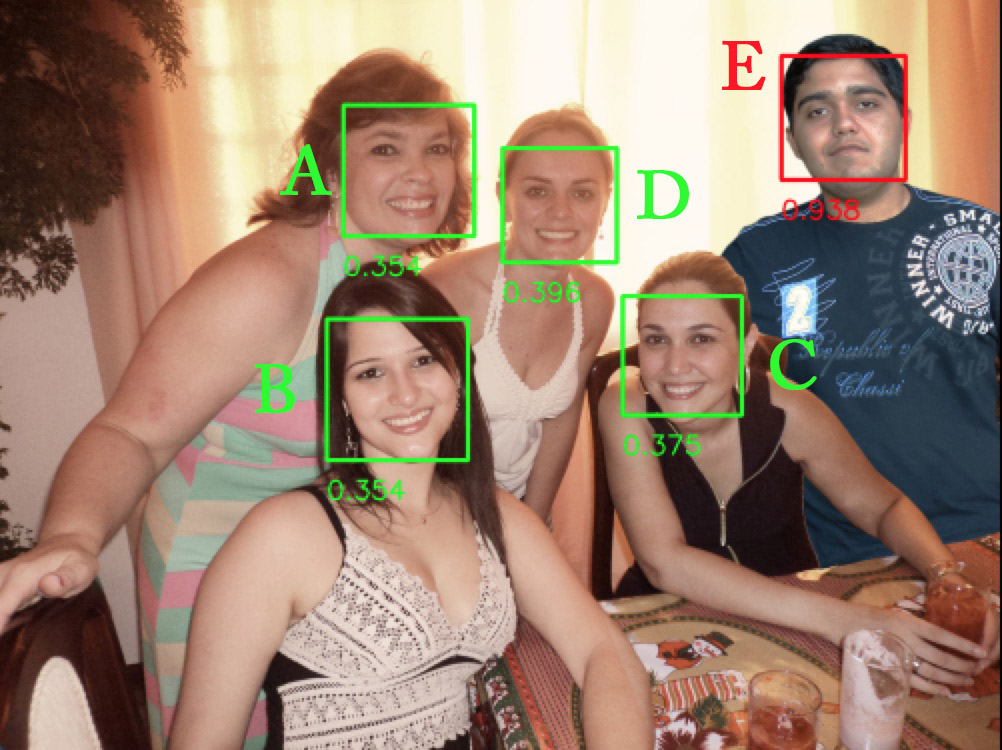
\includegraphics[width=0.8\textwidth]{images/facedetectionoutput_letters.jpg}
\end{center}
\end{column}
\end{columns}
\end{minipage}


\end{tframe}


\begin{tframe}{Regional forgery detection module - 1}
\only<1>{
\begin{center}

\includegraphics[width=1\textwidth]{images/pipeline_regions_1.jpg}
\end{center}
}
\only<2>{
\begin{center}
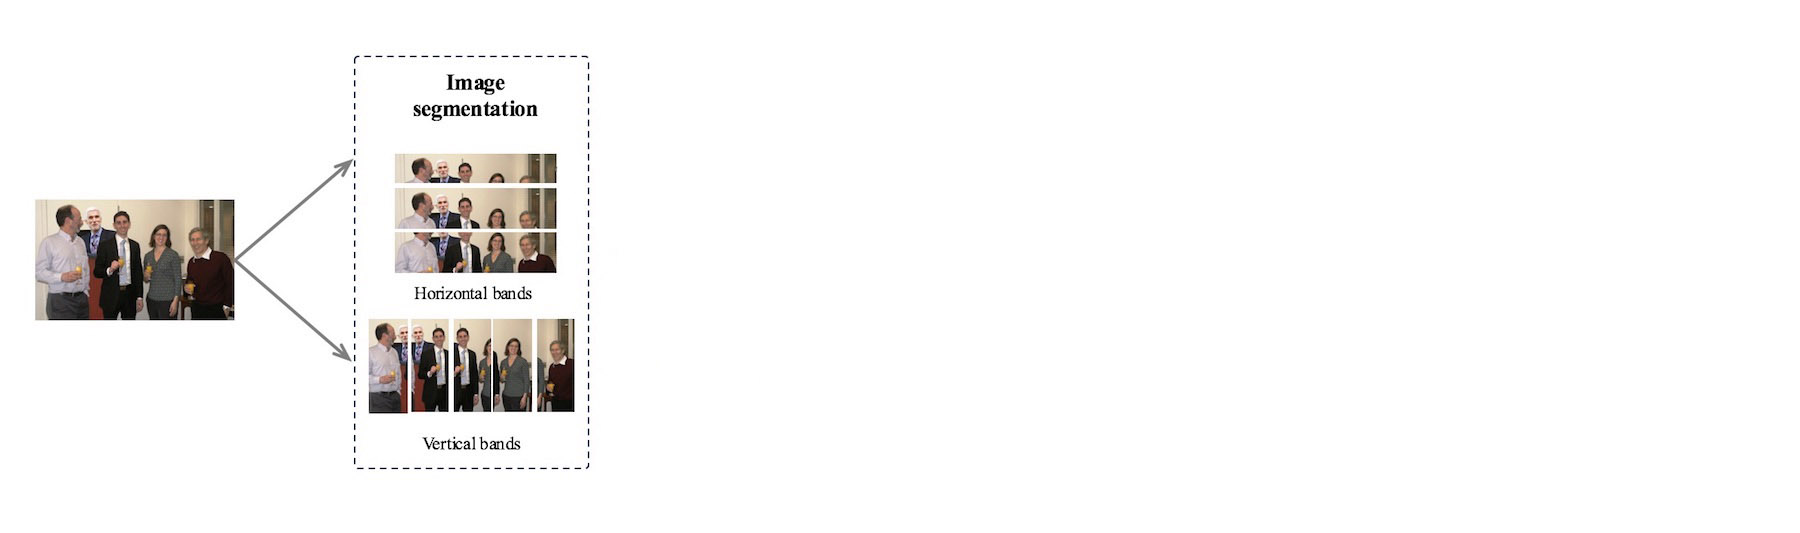
\includegraphics[width=1\textwidth]{images/pipeline_regions_2.jpg}
\end{center}
}
\only<3>{
\begin{center}
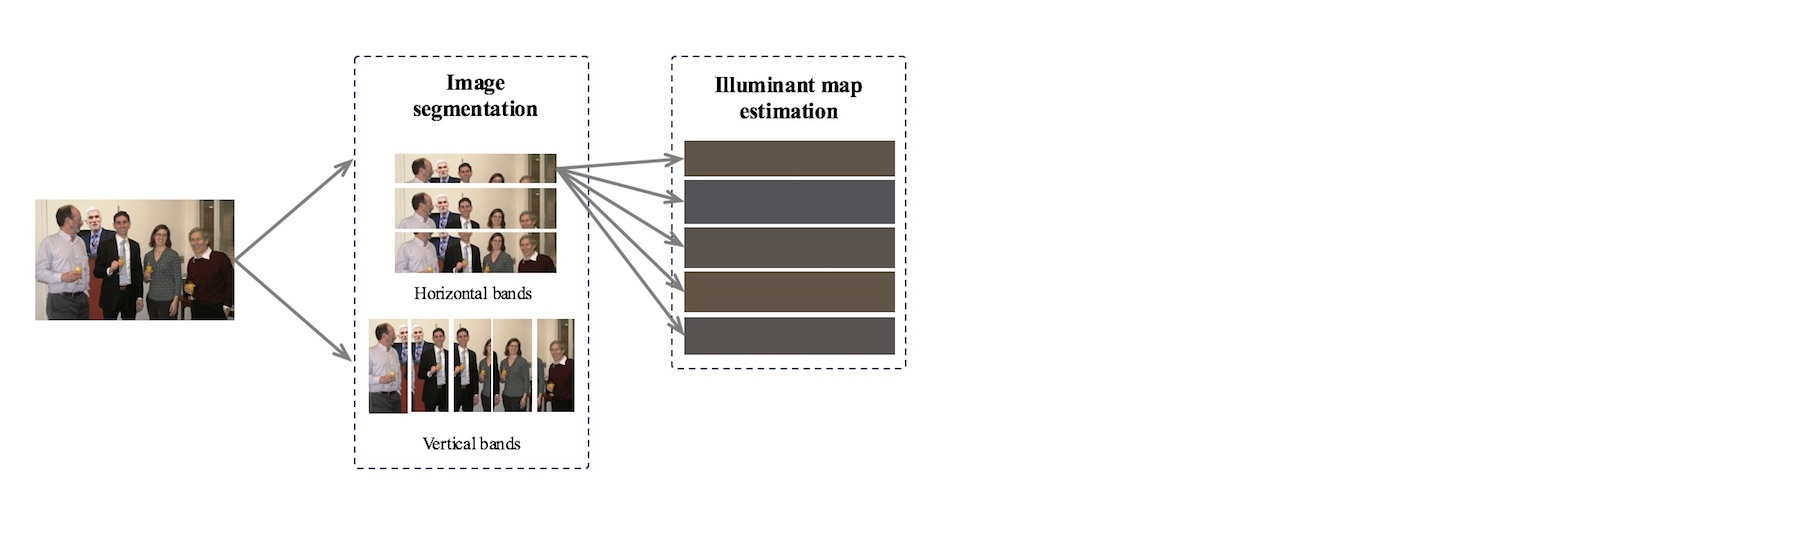
\includegraphics[width=1\textwidth]{images/pipeline_regions_3.jpg}
\end{center}
}
\only<4>{
\begin{center}
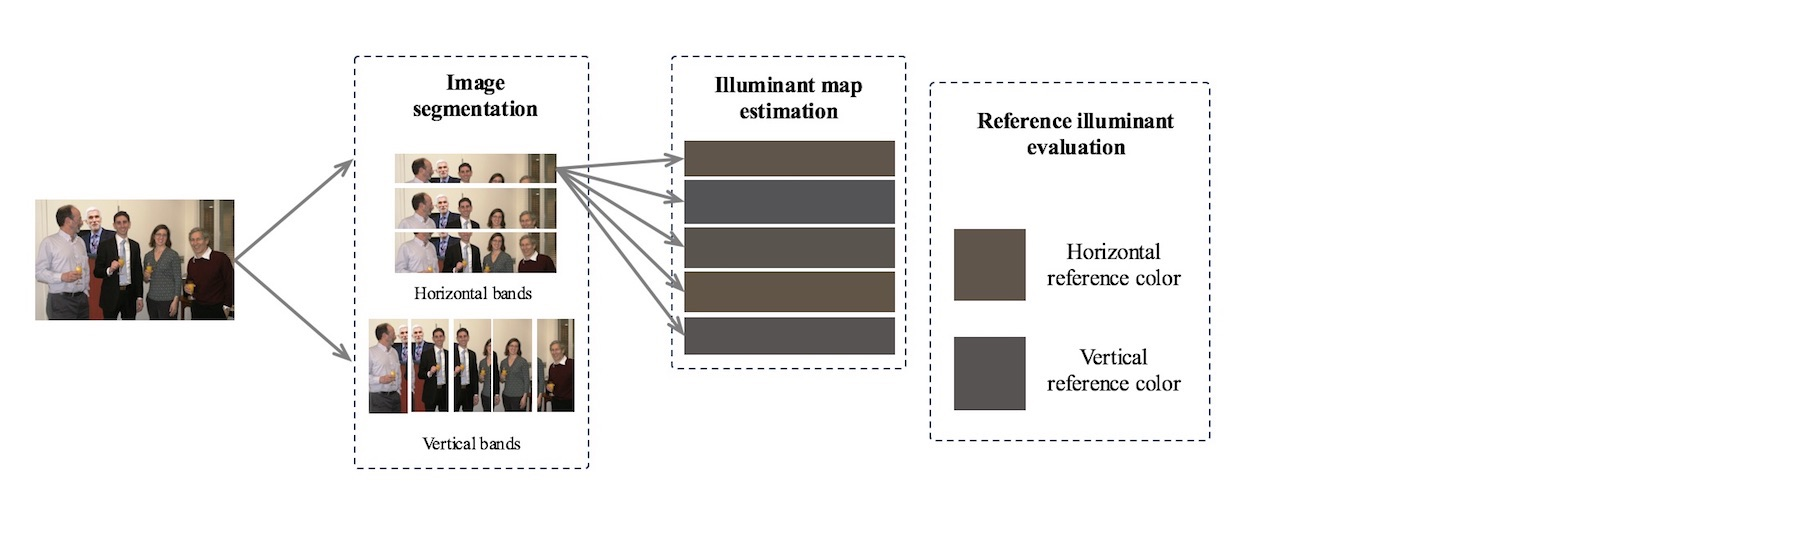
\includegraphics[width=1\textwidth]{images/pipeline_regions_4.jpg}
\end{center}
}
\only<5->{
\begin{center}
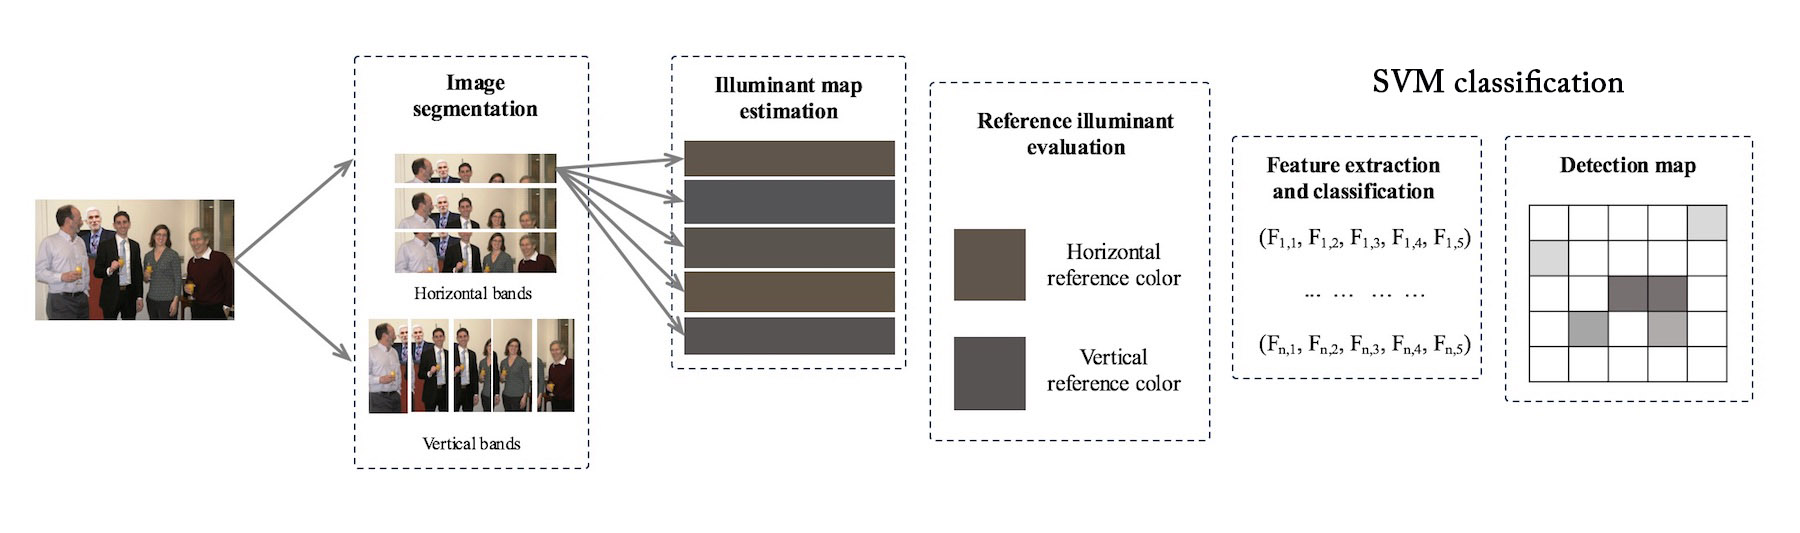
\includegraphics[width=1\textwidth]{images/pipeline_regions_5.jpg}
\end{center}
}

\only<6>{
\vspace{0.2cm}
Two different considered \textbf{reference colors} are considered:
\vspace{0.3cm}
\begin{itemize}
\item \emph{Median}: the median illuminant color for each direction
\vspace{0.1cm}
\item \emph{Global}: the whole image illuminant color
\end{itemize}
}

\end{tframe}

\begin{tframe}{Regional forgery detection module - 2}
\vspace{0.1cm}
The output of the algorithm consist in a \textbf{forgery score} for the image and the forgery \textbf{regional mask}.
\vspace{0.2cm}
\only<1>{
\begin{center}
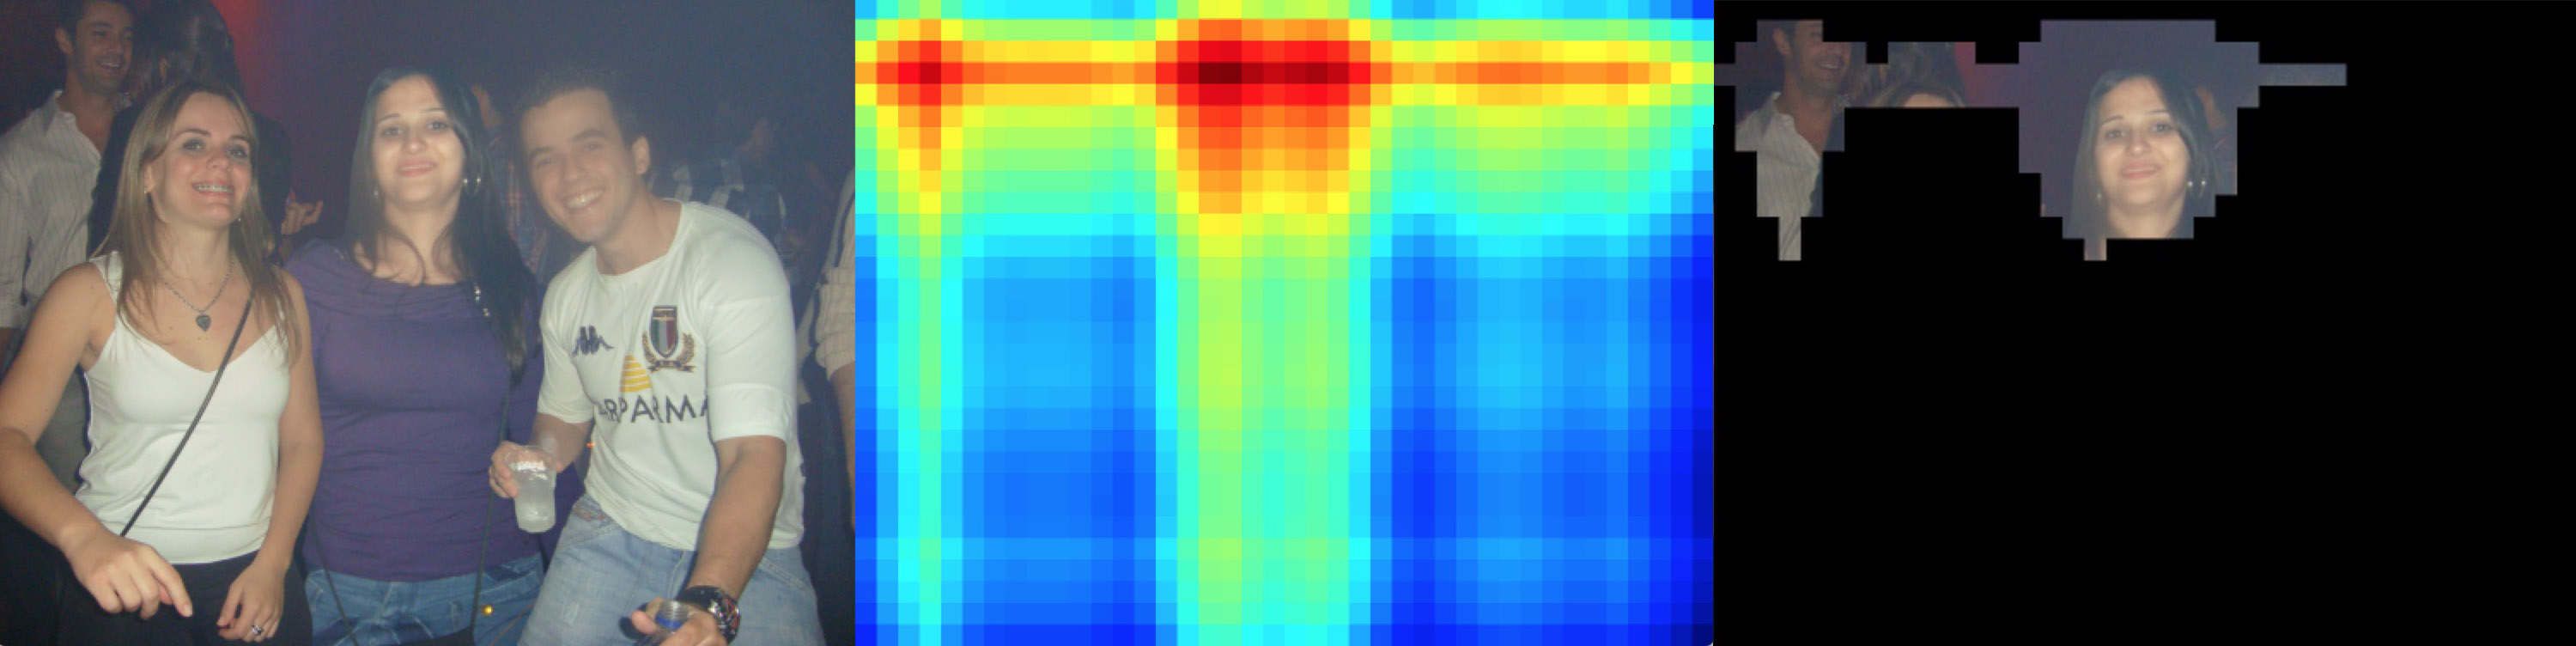
\includegraphics[width=1\textwidth]{images/regionalresult.jpg}
\end{center}
}
\only<2>{
\begin{center}
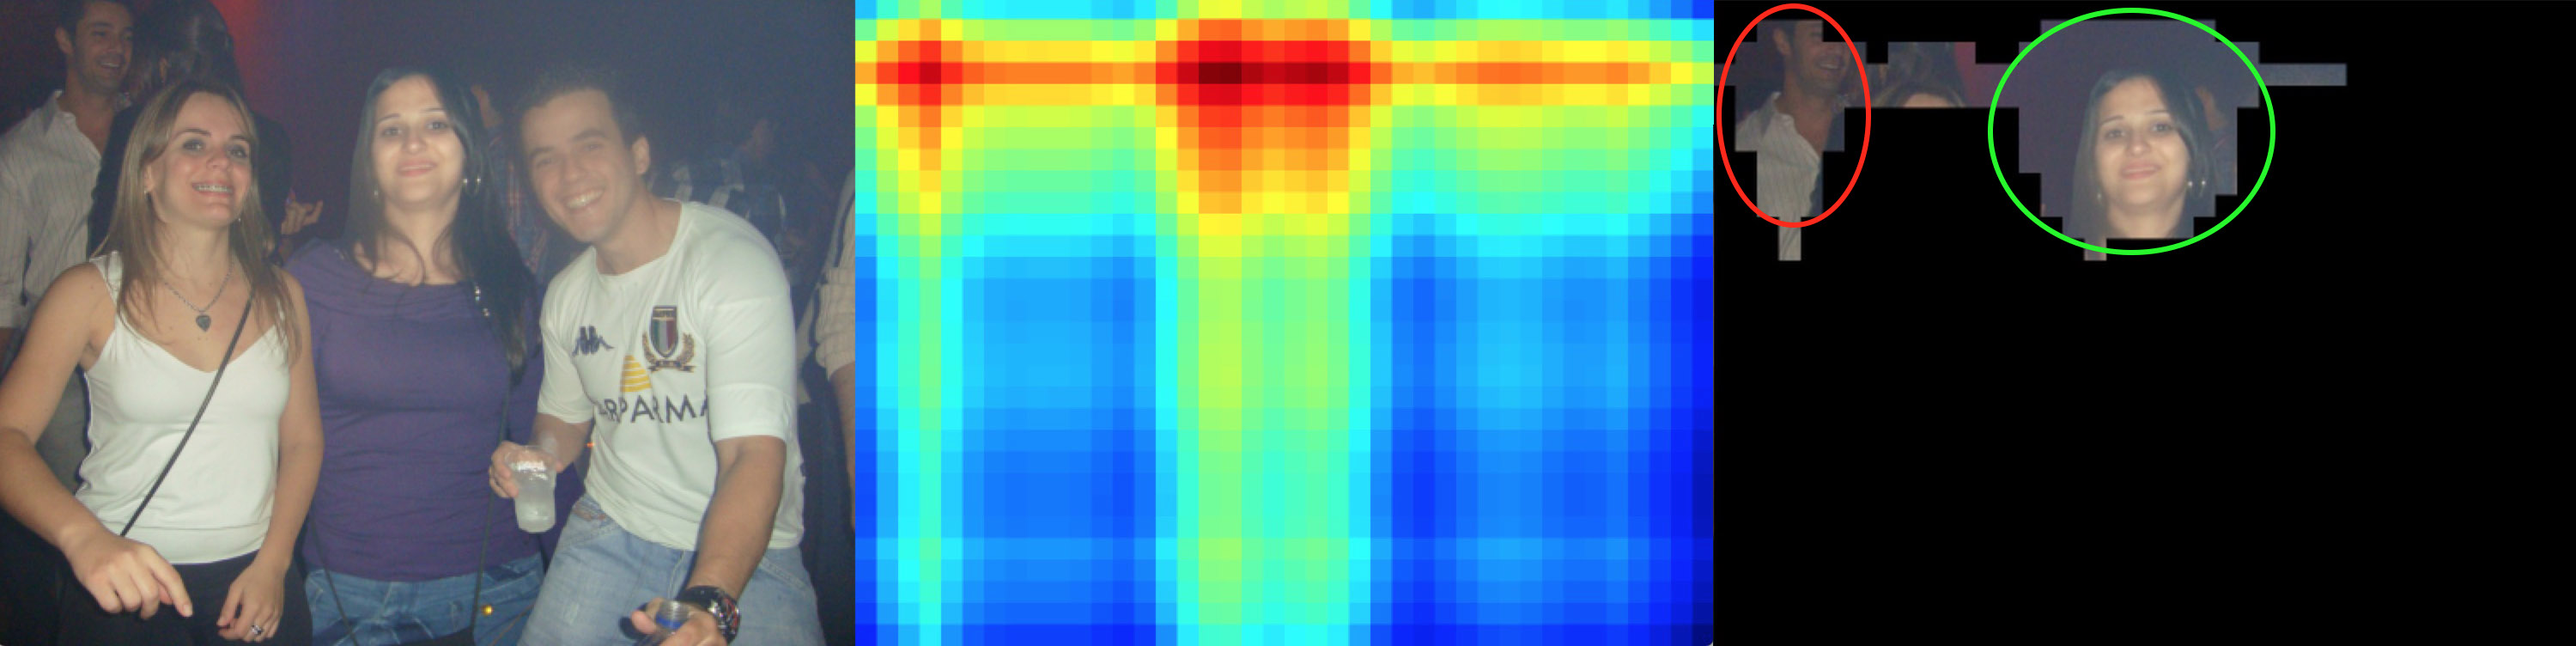
\includegraphics[width=1\textwidth]{images/regionalresult_2.jpg}
\end{center}
}

\vspace{0.2cm}
Work best in presence of \textbf{uniform backgrounds colors} and simple light settings.
\end{tframe}

\begin{tframe}{Evaluation datasets}
\begin{itemize}
\item \textbf{DSO-1}: 200 indoor and outdoor images (100 original and 100 doctored) with an image resolution of 2048 x 1536 pixels.
\vspace{0.1cm}
\item \textbf{DSI-1}: 50 downloaded images (25 original and 25 doctored) with different resolutions. Original images are downloaded from \emph{Flickr}, doctored images collected from different websites.
\end{itemize}
\begin{figure}[!htb]
\minipage{0.5\textwidth}
\centering
  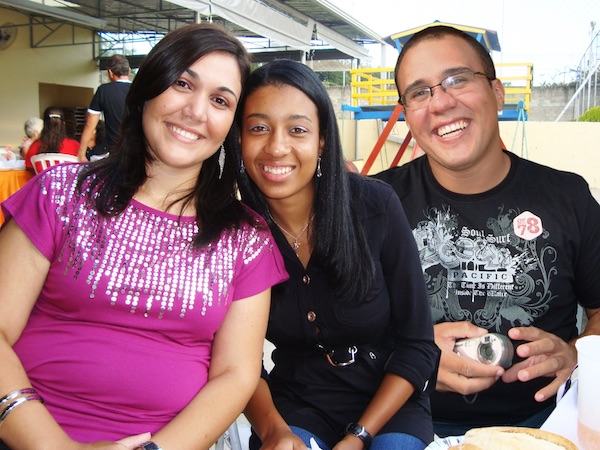
\includegraphics[width=0.6\linewidth]{images/dso_sample_spliced}
  \caption{DSO-1 sample spliced image}\label{fig:dsoimage}
\endminipage\hfill
\minipage{0.5\textwidth}
\centering
  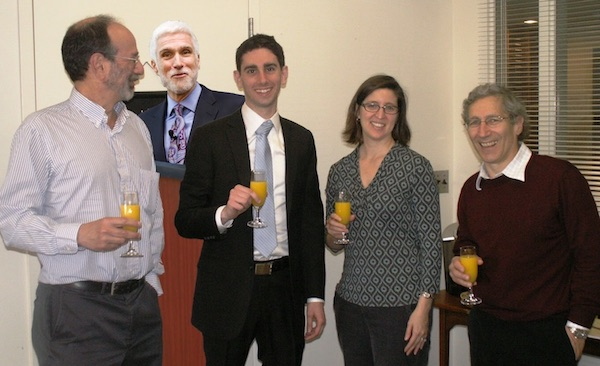
\includegraphics[width=0.7\linewidth]{images/dsi_sample_spliced}
  \caption{DSI-1 sample spliced image}\label{fig:dsiimage}
\endminipage
\end{figure}

\end{tframe}

\begin{tframe}{Experimental results - 1}
Experimental results for face forgery detection module.
\begin{footnotesize}
\begin{table}[h!]
\centering
\begin{tabular}{l c c c c c c c} 
\hline \hline 
\textbf{N.} & \textbf{Train} & \textbf{Test} & \textbf{Faces} & \textbf{PREC} & \textbf{REC} & \textbf{Accuracy} & \textbf{F-Score} \\ [0.5ex]
\hline
1 & DSO-1 & DSO-1 &	540 & 0.58 & 0.89 & 0.81	& 0.64\\
2 & DSI-1 & DSI-1 &	133 & 0.56 & 0.95 & 0.75 & 0.66\\
3 &	DSO-1 & DSI-1 & 540 & 0.41 & 0.18 & 0.63 & 0.25\\ 
4 &	DSI-1 &	DSO-1 &	130 & 0.44 & 0.43 & 0.67 & 0.37\\[1ex]

\hline
\end{tabular}
\caption{Performance of face forgery detection module over single faces using non-uniform weights.}
\label{table:forgerydetections}
\end{table}
\end{footnotesize}
\vspace{0.2cm}
Good results in cross-validation evaluations. In a cross dataset approach, the dataset used for training makes the difference.
\end{tframe}


\begin{tframe}{Experimental results - 2}
Experimental results for regional forgery detection module. 
\begin{footnotesize}
\begin{table}[h!]
\centering
\begin{tabular}{l c c c c c} 
\hline \hline 
\textbf{Test case} & \textbf{Train} & \textbf{RC} & \textbf{ACC} & \textbf{AUC} &\textbf{ F-Score} \\ [0.5ex]
\hline
Test 1 & SplicedCC & Median & 0.54 & 0.53 & 0.26\\
Test 2 & SplicedCC & Global & 0.57 & 0.57 & 0.31\\
Test 3 &	 SplicedDSO & Median & 0.53 & 0.50 & 0.27\\
Test 4 &	 SplicedDSO & Global & 0.61 & 0.63 & 0.33\\ [1ex]
\hline
\end{tabular}
\caption{Performance of region forgery detection module}
\label{table:performanceregionaldet}
\end{table}
\end{footnotesize}
Better results achieved using the\textbf{ global illuminant color }as reference.\\

\vspace{0.2cm}
\textbf{Very low accuracy}: not suitable for a forensic approach.
\end{tframe}

\begin{tframe}{Conclusions}
\begin{itemize}
\vspace{0.1cm}
\item Two different approaches for forgery detection are presented: a face forgery detection module and a generic region forgery detection module.
\vspace{0.1cm}
\item Face module achieved most promising results, but it works only with images involving people forgeries.
\vspace{0.1cm}
\item \textbf{Future developments}: extend the approach to generic objects with composed by similar material.
\vspace{0.1cm}
\item Further improvements can be achieved when more advanced illuminant color estimators become available.
\end{itemize}
\end{tframe}

\begin{tframe}{References}

\begin{footnotesize}

[1] T. Carvalho, et al. "\emph{Illuminant-Based Transformed Spaces for Image Forensics}." IEEE Transactions on Information Forensics and Security 11.4 (2016): 720-733.

\vspace{0.1in}

[2] Y. Fan, P. Carrè, and C. Fernandez Maloigne. \emph{Image splicing detection with local illumination estimation}. In Image Processing ICIP, 2015.

\vspace{0.1in}

[3] J. Van de Weijer, Th. Gevers, A. Gijsenij, \emph{Edge-Based Color Constancy}, IEEE Trans. Image Processing, accepted 2007. 

\vspace{0.1in}

[4] C. Riess and E. Angelopoulou. 2010. \emph{Scene illumination as an indicator of image manipulation}. In \emph{Proceedings of the 12th international conference on Information hiding}, Berlin, Heidelberg, 66-80.

\vspace{0.1in}

[5] S. Gholap and P. Bora. \emph{Illuminant colour based image forensics.} In TENCON IEEE 2008.

\vspace{0.1in}
[6] G. Buchsbaum. \emph{A spatial processor model for object colour perception}. Journal of the Franklin Institute, 1980.

\end{footnotesize}

\end{tframe}

\end{document}